\chapter{Introduction}

Here are summaries of the papers I have read thus far

\section{Background for GAEN keys}
\label{sec:BackgroundGAENKeys}

Background

The first paper is Contact Tracing App Privacy: What Data Is Shared
By Europe’s GAEN Contact Tracing Apps~(\cite{9488728}). This paper discusses the data sent to back end servers of various contact tracing apps in Europe. The apps have two components: the 'client' app which is controlled by the national public health authority and the GAEN service that, on android, is managed by Google as part of the Google Play services. The paper investigates both of these components. It found that the Google Play services component continuously sends requests to the Google servers which contain information such as the phone IMEI, handset hardware serial number, SIM serial number, etc. This may be considered intrusive , however most users would have accepted this data sharing if that had previously enabled Google Play services. This data sharing is not specific to the covid tracing app. There may be a way to identify a user is  specific data is sent in every request. There are experiments run to test the data being sent by different apps. 

The paper CoAvoid: Secure, Privacy-Preserved Tracing of
Contacts for Infectious Diseases~(\cite{9908579}) discusses the privacy and security concerns of covid tracing apps and proposes its own CoAvoid app which improves on these issues. It talks about how inappropriate uses of the GAEN API may expose all information about confirmed patients to servers and relevant users. This may allow someone to gather lots of information about patients and discover their identities, daily routines or social relationships. Due to a limitation of BLE, it may be possible for attackers to send users excess false alarms and put further strain on the public health system (wormhole attack). It talk about how the BLE to calculate if two devices came into contact can be affected by factors such as environment, transmitting power, receiving sensitivity, etc. The GAEN design is vulnerable to profiling, possibly de-anonymising infected persons and wormhole attacks. It describes how the GAEN app works: It randomly generates a Daily Tracking Key (DTK), a unique identifier used for 24 hours. It uses function {\it f} to derive the Rolling Proximity Identifier (RPI) based on the DTK. These identifiers are sent in Bluetooth Advertisements, which will be replaced every 20 minutes. The apps simultaneously collects and stores other users RPIs locally. If a user test positive, their DTK is uploaded to a central server. Other download these DTKs and reconstruct the RPIs. They compare these to their local list of keys. The authenticity of the information being downloaded cannot be verified and thus wormhole attacks may occur. The paper further describes two types of potential attacks: Wormhole and Privacy Analysis attack. It may be possible to identify things about a user by tracking the DTK uploads.

The paper Digital Contact Tracing Solutions: Promises, Pitfalls
and Challenges~(\cite{9931613}) analyses digital contact tracing solutions. It discusses the security and privacy issues with GAEN. It proposes its own solution called TraceCorona. Apple and Google collaborated to create a decentralised contact tracing interface calle Exposure Notification API (GAEN). Access to the API has been given to only one organisation authorised by the government. BLE is used for sensing the proximity between individual devices. The phones send out information like temporary identifiers (TempIDs) that can be sensed by other devices. It also records signal strength in an attempt to estimate the distance of the encounter. It discusses requirements of accuracy, superspreader and accountability for a digital contact tracing system to be acceptable.

The article Privacy and Integrity Threats in Contact
Tracing Systems and Their Mitigations~(\cite{9928557}) reports privacay and integrity threats in GAEN and proposes a new system called Pronto-B2. Threats to security and privacy include the possibility of tracing and deanonymising citizens using passive devices and injecting false at-risk alerts. An attacker may trace a user by linking locations visited by the same user. They may also try to deanonymise users by linking locations visited by users to their real identities. 'Paparazzi Attack': using passive devices, the attacker can catch and store the pseudonyms of a target user. They can link together the passive devices recieved the pseudonyms belonging to the same user. The attacker can obtain information about the habits of an infected user and use it for economical gain. 'Brutus Attack': The attacker colludes with the server and the health authority to discover which user uploaded certain data. Pseudonyms in GAEN are called rolling proximity identifiers (RPIs). A short random secret called Temporary Exposure key (TEK) is generated each day by the smartphone. All RPIs of a given day of a user are generated by running a PRF on the input TEK.

The paper October 2020 Survey of GAEN App Key Uploads~(\cite{survey}) is a survey of the TEKs published across 8 European regions. It estimates the number of users uploading TEKs and compares this to the expected number based on population, number of active users and covid case counts. It reports a shortfall of uploads in a number of regions. The efficacy of these apps remains unclear.

\section{Background for how GAEN keys are Generated}
\label{sec:BackgroundGAENKeysGeneration}
\begin{figure}
    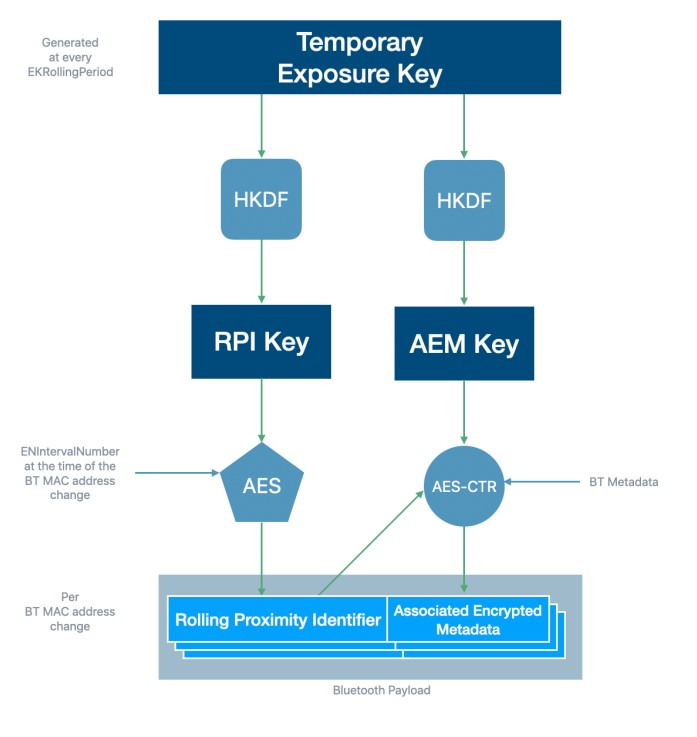
\includegraphics[width=\linewidth]{generatedKEY.jpg}
    \caption{How the GAEN key is generated}
    \label{fig:keyGeneration}
\end{figure}

Here is how the keys are generated. 

The documentation from Google and Apple~(\cite{appleCrypto}) found online details how the GAEN keys are encrypted. An ENIntervalNumber is calculated every 10 minutes, it is a 32-bit unsigned little endian value. The TEKRollingPeriod is how long the Temporary Exposure Key is valid, it is 24 hours. The Temporary Exposure Key is generated and associated with an ENIntervalNumber. It is generated as a 16-byte value using CRNG, which is a cryptographic number generator. At the end of every TEKRollingPeriod, a new key is generated. The Rolling Proximity Identifier Key (RPIK) is derived from the TEK. It is derived by RPIKi ← HKDF(teki, NUL L, UTF8("EN-RPIK"),16), where the HKDF function is as detailed in ~(\cite{rfc5869}), which uses the SHA-256 hash functions. The Rolling Proximity Identifiers are privacy preserving identifiers that are broadcast in Bluetooth payloads. Each time the MAC address changes a new Rolling Proximity Identifier is generated using the Rolling Proximity Identifier Key using RPIi, j ← AES128(RPIKi, PaddedDataj). The use of 16-byte identifiers result in a low probability of collisions and limits the risk of false positive matches. The associated encrypted metadata is encrypted with the Rolling Proximity Identifier. 


\section{Background for Tests for Randomness}
\label{sec:BackgroundTests}

The paper Randomness testing of modern encryption techniques in cloud environment~(\cite{6236554}) compares different modern encryption techniques on a traditional desktop and in a cloud environment. It tests 8 algorithms, including AES which is used in GAEN. It uses the NIST statistical test package which contains 15 tests, listed in the paper. It implements the tests in Java. It runs the NIST tests which produces P-values, which are rejected if they are less than 0.01. There is a max rejection rate, 4 in this paper, there is an equation to calculate this. It runs these tests on all the algorithms and outputs its results. It doesn't find any problems with the algorithms but there are differences when they are ran on the desktop environment versus in the cloud. 

The paper Effectiveness Analysis of Encrypted and Unencrypted Bit Sequence Identification Based on Randomness Test~(\cite{7406118}) uses statistical tests to identify whether a bit sequence is encrypted or unencrypted. Randomness tests are used to evaluate the security of cipher algorithms. It uses the SP800-22 rev1a standard. The standard contains 15 randomness tests but this paper uses 5 of them, frequency test, frequency test within a block, runs test, longest runs of one in a block and cumulative sums test. It provides analysis on some of these tests, frequency, runs, frequency within a block. It describes the P-value used and how it is calculated. It somewhat accurately classifies a bit sequence as encrypted or unencrypted.

The paper Analyzing of Chaos based Encryption with Lorenz and Henon Map~(\cite{8653652})

The paper Statistical Analysis of Enhanced SDEx Encryption Method Based on SHA-512 Hash Function~(\cite{9209663}) performs statistical analysis on an enchanced SDEx method based on the SHA-512 hash function. It uses NIST and carries out four tests: frequency, block frequency, cumulative sum and runs. The algorithm passes all the test, it gets a P-value of > 0.01. It could not do the compression tests from NIST as the size of the test files was too small so it uses WINRAR. It says that of the file is a string of random bits then it should be able to be compressed. It checks that the size of the file before and after compression using WINRAR is the same. The algorithm passes this test also. References a paper about the cryptanalysis of the SDEx method, should read as this paper only does the statistical analysis.

The paper Analysis of the Randomness Performance of the Proposed Stream Cipher Based Cryptographic Algorithm~(\cite{9232553}) does randomness testing on an adapted version of the Vernam Cipher. It uses NIST to do cumulative sums, runs, longest run of ones and frequency tests. It mentions other test suits called NIST STS, Dieharder and TestU01. Mentions Strict Avalanche Criterion (SAC) testing but i do not think this is relevant to the GAEN keys. The cumulative sum is a test concentrates on determining the maximal excursion from zero of the random walk described by the increasing amount of adjusted (-1, +1) digits in the sequence. The Runs Test was utilized to verify whether the total numbers of runs of ones and zeros of various lengths areas projected for a random sequence. The longest run was to define whether the longest run of ones within an M-bit block of the tested sequence is consistent with the length of the longest run of ones anticipated in a random sequence of M bits. For a pseudorandom number generator, the number of ones and zeros in the output must be equal. A test that determines the proportions of zeros and ones for the entire sequence is the Frequency test.

The paper On the Robustness of RSA-OAEP Encryption and RSA-PSS Signatures Against (Malicious) Randomness Failures~(\cite{10.1145/3052973.3053040}) analyses the robustness of the RSA-OAEP encryption scheme and the RSA-PSS signature scheme. The paper gives examples of real world randomness failures but it focused on the enc scheme and signature thing rather than the randmoness of the key itself. It's a very technical paper that I do not fully understand and do not think its discussion of randmoness tests is relevant to the GAEN kesy testing. It is very theoretical. Mentions random oracle model and repeated randmoness and collision resistant? 

The paper Evolving boolean functions for fast and efficient randomness testing~(\cite{10.1145/3205455.3205518}) is VERY USEFUL paper. Introduces a new boolean function for testing randomness, s a novel method for the statistical randomness testing of cryptographic primitives, which is based on the evolutionary construction of the so-called randomness distinguisher. Each distinguisher is represented as a Boolean polynomial in the Algebraic Normal Form. It talks about evolutionary algorithms and their new Boolean functions operating as simple, but high-quality distinguishers of statistical (non)randomness in the data generated by cryptographic algorithms. These boolean functions can provide the same results as the usual test suites NIST etc, but faster and using less data.  The quality of each distinguisher was measured in terms of the so-called Z-score. Mentions another paper using a software package named Ent. In total, they evaluated seven statistics (entropy, compression, hisquared, arithmetic mean, pierror, excess and correlation) associated to five tests, resulting in an observation that studied statistics are not completely independent and could be reduced to five statistics. The paper goes on to describe their function but it is quite confusing and shows their results. Would definitely be worth looking at to test the GAEN keys.

The paper Recommendations on Statistical Randomness Test Batteries for Cryptographic Purposes~(\cite{10.1145/3447773}) is a VERY USEFUL paper. It compares the different batteries(test) suits like NIST, Dieharder, TestU01 and more. It lists the tests used in each one and explains them. It contains very useful references. Need to exam the keys and their structure and refer to this paper to begin deciding on a test suite and what test to run. Contains useful tables of pros and cons of each and compares the tests they have.